\documentclass[floatfix]{article}
\usepackage[utf8x]{inputenc}
\usepackage[pdftex]{graphicx}
\usepackage{mathpazo} 
\usepackage{amsmath}
\usepackage{amsfonts}
\usepackage{amssymb}
\usepackage{braket}
\usepackage{dsfont}
\usepackage[pdftex]{hyperref}   
\usepackage{siunitx}
\usepackage{bbm, dsfont}
\usepackage[font=small]{caption}
\usepackage[margin=1in]{geometry}
\usepackage{float}
\usepackage{tikz}
\usetikzlibrary{arrows,shapes,trees}
\usepackage{media9}

\newcommand*{\gd}{
\textcolor{green}{\ast}}

\newcommand*{\md}{
\textcolor{magenta}{\ast}}

\newcommand*{\ud}{
\underline{\space\space}}

\graphicspath{{images/},{figures/}}

\title{Systems with a strong interaction to an environment}
\author{Eduardo Villase\~nor \\ Carlos Gonzales}
\date{\today}

\begin{document}
\maketitle



\section{Transitions in the P(s)}

We are interested in finding the transitions of from a GOE to Poisson statistics on the
nearest neighbor distribution ($P(s)$) when the parameters change from the ergodic regime to the non-ergodic 
one.

Spectra was obtained with two different methods, in the first one we break the symmetry by varying the Ising interaction between the
spins on the closed chain. For the second one we decomposed the open chain into reflection symmetry sectors.

Animations of the $P(s)$ for a chain in the two cases varying different components of the magnetic kick. As
the color lines in the Fig. \ref{anim_gui} shows.

\begin{figure}[H]
\begin{center}
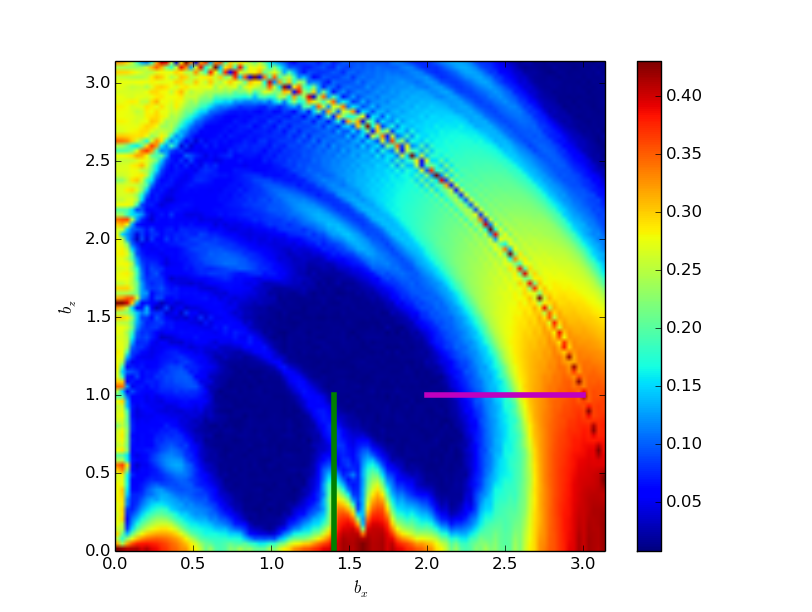
\includegraphics[width=.5\columnwidth]{anim_guide}  
\end{center}
\caption{}
\label{anim_gui}
\end{figure}

The animations are ass follows 
\begin{itemize}
\item ``Ps\ud transition1" - Closed chain $J=1$ $b_x=[2,3]$ $b_z=1.$ $\Delta J = 0.1$ $\md$
\item ``Ps\ud transition1\underline{\space\space}sym" - Open chain $J=1$ $b_x=[2,3]$ $b_z=1.$ reflection symmetries used $\md$
\item ``Ps\ud transition2" - Closed chain $J=1$ $b_x=1.4$ $b_z=[0,1]$ $\Delta J = 0.1$ $\gd$
\item ``Ps\ud transition2\underline{\space\space}sym" - Closed chain $J=1$ $b_x=1.4$ $b_z=[0,1]$ reflection symmetries used $\gd$
\end{itemize}

Comparin the two methods we see that breaking symmetries using small variations in the Ising interaction in the chain gives
a better shaped $P(s)$. Also the transitions shows some correlation with the map \ref{anim_gui} only in some places of the
regime, this remains a mystery


\section{Purity decay}

We start by studying ``model3" and ``model4" (see ``models.cu"). Our first analysis is made with the parameters that make 
both systems $A$ and $B$ ergodic. The parameters are $[J_c,J_p,J_s,\Delta J,\Delta b, b_x, b_z]$

Where:
\begin{itemize}
\item $J_c$ - Interaction of $C$ with $A$.
\item $J_p$ - Interaction between $A$ and $B$.
\item $J_s$ - Center of internal interactions of $A$ and $B$.
\item $\Delta J$ - Such that $J_i \in [J_s - \Delta J, J_s + \Delta J]$.
\item $\Delta b$ - Such that $b_{{\{x,z\}}_i} \in [b_\{x,z\} - \Delta b, b_\{x,z\} + \Delta b]$.
\item $b_x$ - Center of magnetic component $x$.
\item $b_z$ - Center of magnetic component $z$. 
\end{itemize}

We fix all parameters except $J_p$ and we calculate an average of the purity defined as:
\begin{equation}
<\gamma>_{T_1}^{T_2} = \frac{1}{T_2-T_1+1} \sum_{t=T_1}^{T_2} \gamma(t).
\end{equation}

For $<\gamma>_{80}^{100}$ using the parameters $J_c,J_p,J_s,\Delta J,\Delta b,b_x,b_z=[0.05,0.,1.0,0.1,0,1.0,1.0] $ 
and $J_p \in [0,2\pi]$. ${\rm dim}([A,B,C])=[4,8,1]$.

For ``model3" - ``model3\ud open" we obtain

\begin{figure}[H]
\begin{center}
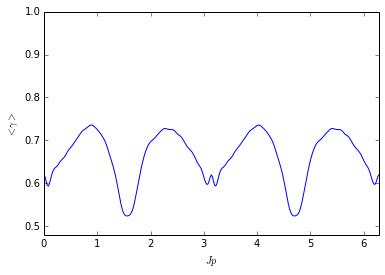
\includegraphics[width=.48\columnwidth]{p_model3}  
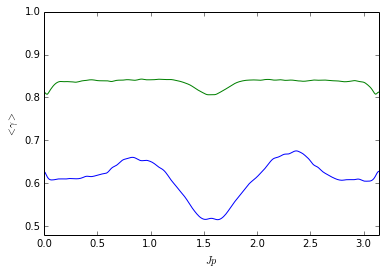
\includegraphics[width=.48\columnwidth]{p_model3_open}  
\end{center}
\caption{}
\label{p_m3}
\end{figure}




With the same parameters for ``model4" - ``model4\ud open"

\begin{figure}[H]
\begin{center}
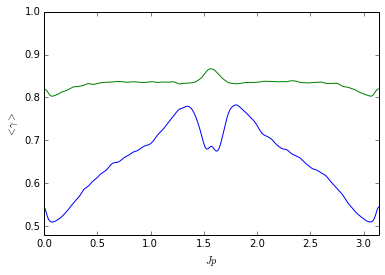
\includegraphics[width=.48\columnwidth]{p_model4}  
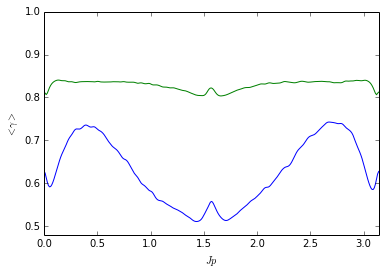
\includegraphics[width=.48\columnwidth]{p_model4_open}  
\end{center}
\caption{}
\label{p_m4}
\end{figure}

% Something very important is noted between these two figures. In Fig. \ref{p_m3} we see the maximum of $<\gamma>$ around
% the value $J_p=1.0$ which is almost equivalent as one central system connected to a large system, as $A$ and $B$ merge into one big chain.
% In Fig. \ref{p_m4} we see however that is not the case and one can achieve very high values of $<\gamma>$ for a certain small value of 
% $J_p$.

The big question this first result show is that,  how much topology of the system plays a central role in the conservation of the purity? If so how about the interaction of $A$ and $B$?
Or if we add a fourth system $D$?.

First question.
With the same parameters for ``model5" - ``model5\ud open"  ${\rm dim}([A,B,C])=[6,6,1]$.

\begin{figure}[H]
\begin{center}
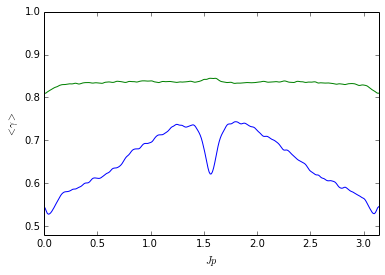
\includegraphics[width=.48\columnwidth]{p_model5}  
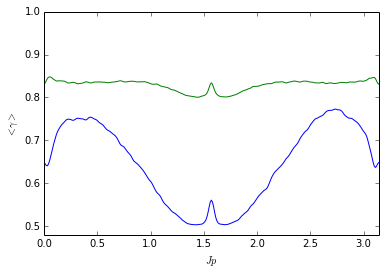
\includegraphics[width=.48\columnwidth]{p_model5_open}  
\end{center}
\caption{}
\label{p_m4}
\end{figure}


Second question.
With the same parameters for ``model6" - ``model6\ud open"

\end{document}

